\documentclass[12pt,letterpaper]{article}
\usepackage[spanish]{babel}
\usepackage[utf8]{inputenc}
\usepackage{graphicx}
\usepackage{pst-pdf}
\usepackage{amssymb}
\usepackage{hyperref}
\usepackage{listings}
\usepackage{biblatex}
\addbibresource{tarea_5.bib} 
\title{{Programacion estructurada.}}
\author{Daniel Reyes Barrera}
\date{23 de noviembre de 2020}

\begin{document}
\maketitle

\abstract{En este documento se han resuelto algunos problemas computacionales utilizando las herramientas aprendidas en la clase 5 – Programaci\'on estructurada del curso de programaci\'on C++, como son Modularizaci\'on, m\'etodos y funciones las cuales nos proporcionan un mejor uso para un bloque recurrente de instrucciones.



\section{Ejercicio 1.}

Escriba un programa que imprima un men\'u para seleccionar un tipo de figura geom\'etrica de la siguiente forma:
\begin{figure}[ht!]
  \centering
  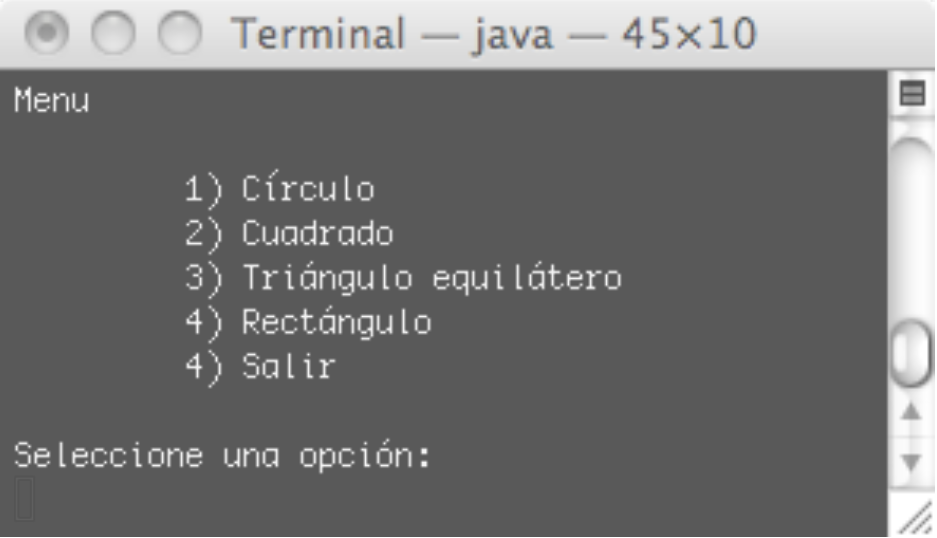
\includegraphics[width=0.6\textwidth]{figures/captura}
\end{figure}

El usuario debe seleccionar una opci\'on y el programa debe calcular el \'area y per\'imetro de la opci\'on seleccionada. Programe cada opci\'on en un m\'etodo independiente. El programa debe regresar al menu principal hasta que el usuario seleccione la opci\'on salir.

\subsection{Problema computacional.}
\textbf{Objetivo:} Calcular \'areas de figuras deseadas de manera indefinida.

\textbf{Entrada:} Un n\'umero que represente la figura deseada y posteriormente sus dimensiones.

\textbf{Salida:} El area de la figura deseada.

\subsection{Algoritmo.}
Para solucionar el problema computacional, programamos el algoritmo dentro del ciclo de repetici\'on \texttt{do-while} para que se siga ejecutando hasta que el usuario decida salir. Cada opci\'on del calculo de \'areas se programo  m\'etodos diferentes.

El código fuente está disponible en mi repositorio de git hub. \cite{url:calcular_area}

\subsection{Instancia del problema.}
Como prueba de escritorio, se seleccionaron las siguientes instancias del problema.Se calcularon las siguientes \'areas: Un circulo de radio 4 y el \'area de un rectangulo de base = 2 y altura = 5. . La salida del programa se observa en la Figura \ref{fig:calcular_area}.
\begin{figure}[ht!]
  \centering
  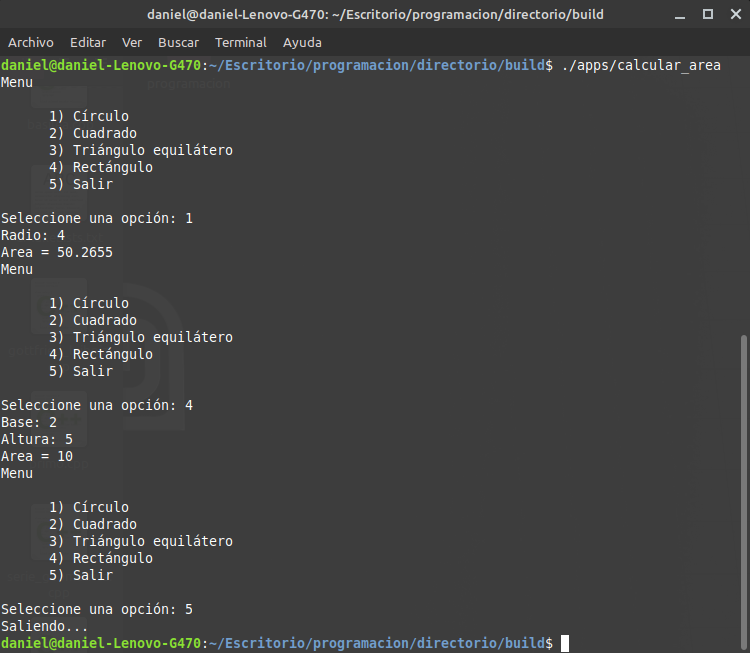
\includegraphics[width=0.8\textwidth]{figures/calcular_area}
  \caption{Ejecución de algunas instancias del problema.}
  \label{fig:calcular_area}
\end{figure}

\newpage

\section{Ejercicio 2.}

El m\'aximo com\'un divisor de dos enteros es el entero m\'as grande que puede dividir a cada uno de los dos n\'umeros. Programe el algoritmo para calcular el m\'aximo com\'un divisor en un m\'etodo independiente.

\subsection{Problema computacional.}
\textbf{Objetivo:} Dado dos n\'umero enteros calcular el m\'aximo comun divisor.

\textbf{Entrada:} Dos n\'umeros enteros.

\textbf{Salida:} El valor de MCD de ambos n\'umeros introducidos.

\subsection{Algoritmo.}
Para solucionar el problema computacional, utilizaremos el algorimo de Euclides \cite{url:euclides} que consiste en tomar en cuenta la parte entera de la divisi\'on de los n\'umeros (cociente) y su parte residual (resto), si el resto no es cero volvemos a dividir el divisor entre el cociente, aplicamos ese m\'etodo hasta que el resto sea igual a 0 y entonces el ultimo divisor es el MCD.


El código fuente está disponible en mi repositorio de git hub. \cite{url:MCD}

\subsection{Instancia del problema.}
Como prueba de escritorio, se seleccionaron las siguientes instancias del problema. Entrada: $a=45 $, $b=50$ y $a=1032$, $b=180$. La salida del programa se observa en la Figura \ref{fig:MCD}.
\begin{figure}[ht!]
  \centering
  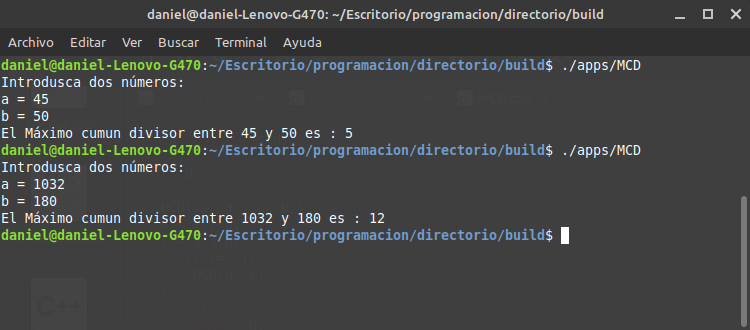
\includegraphics[width=0.8\textwidth]{figures/MCD}
  \caption{Ejecución de algunas instancias del problema.}
  \label{fig:MCD}
\end{figure}

\newpage

\section{Ejercicio 3.}

Programe el algoritmo para determinar si el n\'umero es pal\'indromo y el algoritmo para validar la entrada en m\'etodos independientes.
Sugerencia: Haga uso de los operadores m\'odulo y divisi\'on para separar el n\'umero tecleado en unidades, decenas, centenas, etc.

\subsection{Problema computacional.}
\textbf{Objetivo:} Dado un n\'umero entero determinar si es pal\'indromo.

\textbf{Entrada:} Un n\'umero entero mayor que 0.

\textbf{Salida:} La respuesta de si el n\'umero dado es o no pal\'indromo.

\subsection{Algoritmo.}
Para solucionar el problema computacional, utilizamos una variable de apoyo para comparar el n\'umero dado mediante la separaci\'on en unidades, decenas, centenas, etc. Utilzando los operadores m\'odulo y divisi\'on.


El código fuente está disponible en mi repositorio de git hub. \cite{url:palindromo}

\subsection{Instancia del problema.}
Como prueba de escritorio, se seleccionaron las siguientes instancias del problema. Entrada: 12344321, 2234321, 76567 y 12324. La salida del programa se observa en la Figura \ref{fig:palindromo}.
\begin{figure}[ht!]
  \centering
  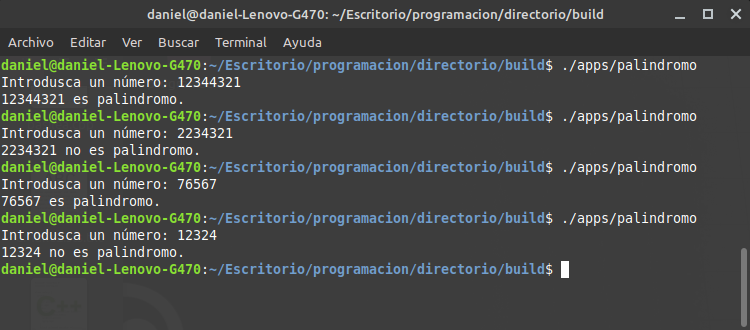
\includegraphics[width=0.8\textwidth]{figures/palindromo}
  \caption{Ejecución de algunas instancias del problema.}
  \label{fig:palindromo}
\end{figure}

\section{Ejercicio 4.}

Programe el algoritmo de Schrage para generar n\'umeros pseudo-aleatorios
entre $0$ y $m$.
El j-\'esimo elemento de la sucesi\'on de n\'umeros pseudo-aleatorios, denotado por $I_j$ , se calcula con la siguiente ecuaci\'on:
$$ I_j = a(I_{j-1} mod \ m) $$
$$I_{j}=\left\lbrace\begin{array}{c} a(I_{j-1} mod \ q)-r[I_{j-1} /q] \ \ \ si \ a(I_{j-1} mod \ q )-r[I_{j-1}/q > 0] \\ a(I_{j-1} mod \ q)-r[I_{j-1} /q] + m \ \ \ \ \ \ \ \ en \ otro \ caso \ \ \ \ \ \ \ \ \  \ \ \ \ \ \end{array}\right.  $$

donde $a = 75$, $m = 2^{31}-1$, $q = 127773$, $r = 2836$ y $I_0$ es la semilla del generador, cuyo valor se deja a criterio del programador. Los corchetes indican que el resultado de la divisi\'on se trunca para obtener solamente la parte entera.


\subsection{Problema computacional.}
\textbf{Objetivo:} Calcular una cantidad n de n\'umeros aleatorios dados por el usuario.

\textbf{Entrada:} Un n\'umero entero mayor que 0.

\textbf{Salida:} Una sucesi\'on de n\'umeros aleatorios.

\subsection{Algoritmo.}
Para solucionar el problema computacional, seguimos las instrucciones del algoritmo de Schrage \cite{url:rage}. Escogiendo $I_0 = 1234567$ como el valor de la semilla


El código fuente está disponible en mi repositorio de git hub. \cite{url:schrage}

\subsection{Instancia del problema.}
Como prueba de escritorio, se seleccionaron las siguientes instancias del problema. Entrada: $n = 23$. La salida del programa se observa en la Figura \ref{fig:schrage}.
\begin{figure}[ht!]
  \centering
  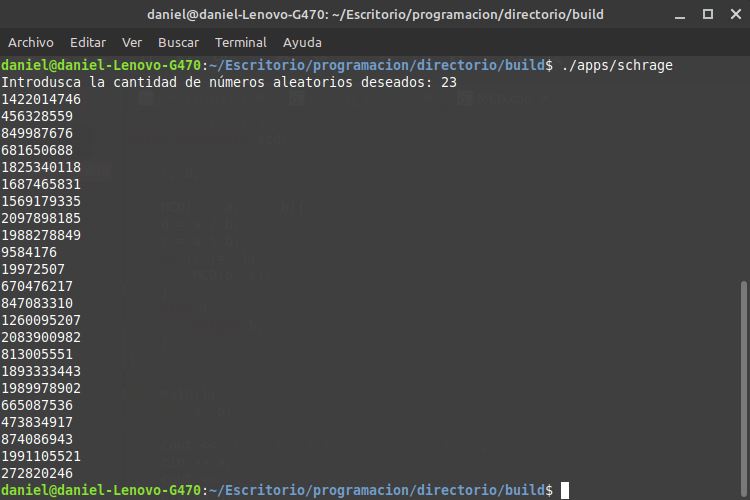
\includegraphics[width=0.8\textwidth]{figures/schrage}
  \caption{Ejecución de algunas instancias del problema.}
  \label{fig:schrage}
\end{figure}


\newpage


\section{Conclusiones.}
En algunas ocaciones la recursividad puede ser una herramienta practiva al programar alg\'un algoritmo en vez de utilizar ciclos \texttt{for} o \texttt{while}, aunque sea menos intuitivo que los ciclos, es m\'as practico y util en muchos problemas. La declaraci\'on de m\'etodos o funciones tambien son una herramienta imprescindible al programar ya que al reutilizar bloques enteros de c\'odigos en distintas partes de nuestro programa nos ahorra tiempo y varias lineas de c\'odigo.

\printbibliography 


\end{document}
